\problemname{DFS}

You might already be familiar with the famous DFS (depth-first search) algorithm
for traversing a graph. In this problem, we will only consider connected
undirected simple graphs (without loops and parallel edges) with vertices
numbered $0, 1, \ldots, n-1$, and the DFS algorithm will output depths and
vertices as follows:

\begin{verbatim}
DFS(d, v):
    output d/v
    mark vertex v as visited
    W = the list of neighbors of v ordered by increasing numbers
    for each w in W:
        if vertex w has not yet been visited:
            DFS(d + 1, w)
\end{verbatim}

Write a program that outputs the number of different graphs for which the call
\texttt{DFS(0, n - 1)} produces the same printout as the one given on the input.
For example, the output

\begin{verbatim}
0/2
1/0
2/1
\end{verbatim}

is produced by calling \texttt{DFS(0, 2)} on either of the following two
connected undirected simple $3$-vertex graphs:

\begin{figure}[h]
  \centering
  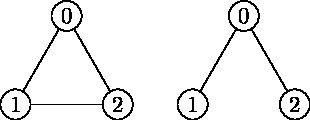
\includegraphics[width=0.45\textwidth]{dfs-graphs}
\end{figure}

\section*{Input}
The input is the output of the call \texttt{DFS(0, n - 1)} on an unknown
$n$-vertex connected undirected simple graph. The input thus consists of $n$
lines in the format \texttt{d/v}, with the first line being \texttt{0/n-1}.

The following limits hold:
\begin{itemize}
  \item $1 \leq n \leq 2 \cdot 10^5$
\end{itemize}

\section*{Output}
Print the number of different graphs with the required property. Because this
number can be very large, output the result modulo $1\,000\,000\,007$.

\section*{Scoring}
Your solution will be tested on a set of test groups.
To earn points for a group, you must pass all test cases in that group.

\noindent
\begin{tabular}{| l | l | p{12cm} |}
  \hline
  \textbf{Group} & \textbf{Points} & \textbf{Constraints} \\ \hline
  $1$ & $10$ & $n \leq 6$ \\ \hline
  $2$ & $20$ & $n \leq 500$ \\ \hline
  $3$ & $20$ & $n \leq 10^4$ \\ \hline
  $4$ & $10$ & For each $i \in \{2, \ldots, n\}$, the $i$-th input line is
               \texttt{i-1/i-2}. \\ \hline
  $5$ & $20$ & For each $i \in \{2, \ldots, n\}$, the $i$-th input line is
               \texttt{i-1/v} for some $v \in \{0, \ldots, n-2\}$. \\ \hline
  $6$ & $20$ & No additional constraints. \\ \hline
\end{tabular}
